\textbf{Challenge Question} A gambler has the opportunity to make bets on
the outcomes of a sequence of coin flips. If the coin comes up heads, she wins as many
dollars as she has staked on that flip; if it is tails, she loses her stake. The game ends
when the gambler wins by reaching her goal of \$100, or loses by running out of money.
On each flip, the gambler must decide what portion of her capital to stake, in integer
numbers of dollars. This problem can be formulated as an undiscounted, episodic, finite
MDP. The state is the gambler's capital, $s \in \{1, 2,..., 99\}$ and the actions
are stakes, $a \in \{0, 1,..., \min(s, 100-s) \}$.
The reward is +1 when reaching the goal of \$100 and zero on all other transitions.

\begin{enumerate}
  \item Let $p_{h}$ denote the probability of heads. Then the figure below illustrates an optimal policy for $p_{h} = 0.4$.
    Describe the strategy found by the optimal policy.
  \item How does the optimal policy change when $p_{h}$ is equal to, higher than or lower than $0.5$?
\end{enumerate}

\begin{figure}[h!]
  \center
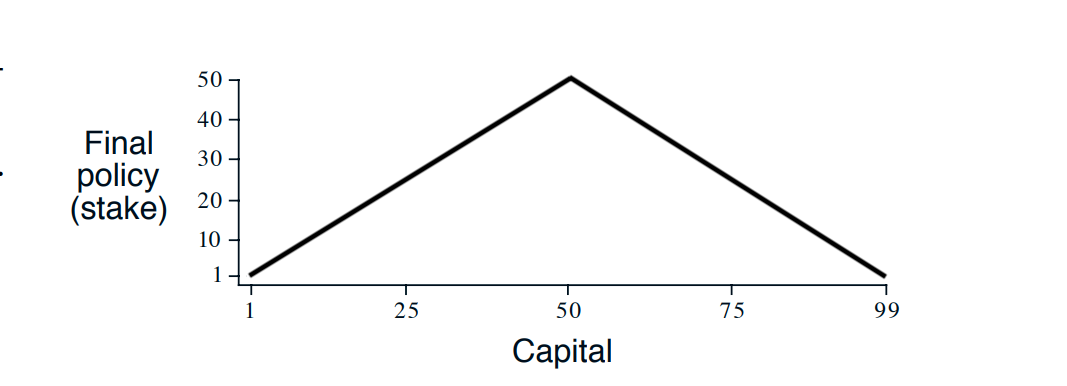
\includegraphics[width=0.9\linewidth]{figures/figure_4dot3_mod.png}
\end{figure}
\bigspace